\def\year{2017}\relax
\documentclass[letterpaper]{article}
\usepackage{aaai17}
\usepackage{times}
\usepackage{helvet}
\usepackage{courier}

% Packages added by Rob
% Also: grffile, latexsym, textcomp, longtable, booktabs, amsmath, amsfonts, amssymb?
\usepackage{amsmath}
\usepackage[utf8]{inputenc}
\usepackage{url}
\usepackage{graphicx}
\providecommand{\tightlist}{\setlength{\itemsep}{0pt}\setlength{\parskip}{0pt}}%

% Packages added by Josh
\usepackage{amsmath}

\frenchspacing
\setlength{\pdfpagewidth}{8.5in}
\setlength{\pdfpageheight}{11in}
\pdfinfo{
/Title (Insert Your Title Here)
/Author (Put All Your Authors Here, Separated by Commas)}
\setcounter{secnumdepth}{0}
\begin{document}

\title{ConceptNet 5.5: An Open Multilingual Graph of General Knowledge}
\author{
    Robert Speer \\ Luminoso Technologies, Inc. \\ 675 Massachusetts Ave. \\ Cambridge, MA 02139
    \And
    Joshua Chin \\ Union College \\ 807 Union St. \\ Schenectady, NY 12308
}

\maketitle


\section{Abstract}\label{abstract}

Machine learning about language can be improved by supplying it with specific knowledge and sources of external information. We present here a new version of the linked open data resource ConceptNet that is particularly well suited to be used with modern NLP techniques such as word embeddings.

ConceptNet is a knowledge graph that connects words and phrases of natural language with labeled edges. Its knowledge is collected from many sources that include expert-created resources, crowd-sourcing, and games with a purpose. It is designed to represent the general knowledge involved in understanding language, improving natural language applications by allowing the application
to better understand the meanings behind the words people use.

When ConceptNet is combined with word embeddings acquired from distributional semantics (such as word2vec), it provides applications with understanding that they would not acquire from distributional semantics alone, nor from narrower resources such as WordNet or DBPedia. We demonstrate this with state-of-the-art results on intrinsic evaluations of word relatedness that translate into improvements on applications of word vectors, including solving SAT-style analogies.


\section{Introduction}\label{introduction}

ConceptNet is a knowledge graph that connects words and phrases of
natural language (\emph{terms}) with labeled, weighted edges
(\emph{assertions}). The original release of ConceptNet \cite{liu2004conceptnet}
was intended as a parsed representation of Open Mind Common Sense
\cite{singh2002omcs}, a crowd-sourced knowledge project. This paper
describes the release of ConceptNet 5.5, which has expanded to include
lexical and world knowledge from many different sources in many
languages.

ConceptNet represents relations between words such as:

\begin{itemize}
    \item \emph{Fire} is \emph{hot}.
    \item A \emph{net} is used for \emph{catching fish}.
    \item ``\emph{Leaves}'' is a form of the word ``\emph{leaf}''.
    \item The word \emph{cold} in English is \emph{studený} in Czech.
    \item Um \emph{alimento} é usado para \emph{comer} [Food is used for eating].
\end{itemize}

In this paper, we will concisely assertions such as the above as triples of
their start node, relation label, and end node: the assertion that ``a dog has
a tail'' can be represented as (\emph{dog}, \emph{HasA}, \emph{tail}).

ConceptNet also represents links between knowledge resources. In addition to
its own knowledge about the English term \emph{astronomy}, for example,
ConceptNet contains links to URLs that define \emph{astronomy} in WordNet,
Wiktionary, UMBEL, and DBPedia.

The graph-structured knowledge in ConceptNet can be particularly useful to NLP
learning algorithms, particularly those based on word embeddings, such as
\cite{mikolov2013word2vec}. We can use ConceptNet to build semantic spaces that
are more effective than distributional semantics alone.

The most effective semantic space is one that learns from both distributional
semantics and ConceptNet, using a generalization of the ``retrofitting'' method
\cite{faruqui2015retrofitting}. We call this hybrid semantic space ``ConceptNet
Numberbatch'', to clarify that it is a separate artifact from ConceptNet
itself.

ConceptNet Numberbatch performs significantly better than other systems across
many evaluations of word relatedness, and this increase in performance
translates to improvements on downstream tasks such as analogies.  On Turney's
corpus of SAT-style analogy questions \cite{turney2005lra}, its accuracy of
56.4\% is slightly higher than the previous best system (Turney's LRA) and only
slightly lower than the performance of the average human test-taker.

Building word embeddings is not the only application of ConceptNet, but it is a
way to apply ConceptNet that achieves clear benefits and is compatible with
ongoing research in distributional semantics. This shows the continued relevance of
ConceptNet, and of explicitly collecting knowledge to improve the computational
understanding of semantics.

In this paper, we will begin by describing ConceptNet 5.5 and its features,
show how to use ConceptNet alone as a semantic space and a measure of word
relatedness, and then proceed to describe and evaluate the hybrid system
ConceptNet Numberbatch on these various semantic tasks.

\section{Structure of ConceptNet}\label{structure-of-conceptnet}

\subsection{Knowledge sources}\label{knowledge-sources}

ConceptNet 5.5 is built from the following sources:

\begin{itemize}
\item
  Facts acquired from Open Mind Common Sense (OMCS) \cite{singh2002omcs}
\item
  Information extracted from parsing Wiktionary, in multiple languages,
  with a custom parser (``Wikiparsec'')
\item
  ``Games with a purpose'' designed to collect common knowledge,
  including Verbosity \cite{vonahn2006verbosity} in English, nadya.jp
  \cite{nakahara2011nadya} in Japanese, and the PTT Pet Game
  \cite{kuo2009petgame} in Chinese
\item
  Open Multilingual WordNet \cite{bond2013linking}, a linked-data
  representation of WordNet \cite{miller1998wordnet} and its parallel
  projects in multiple languages, representing word meanings as
  ``synsets'' of synonymous word senses
\item
  JMDict \cite{breen2004jmdict}, a Japanese-multilingual dictionary
\item
  OpenCyc \cite{matuszek2006cyc}, a hierarchy of hypernyms provided by
  Cyc, a system that represents common sense knowledge in predicate
  logic, and includes connections to the UMBEL ontology
  \cite{bergman2008umbel}
\item
  A subset of DBPedia \cite{auer2007dbpedia}, a network of facts
  extracted from Wikipedia infoboxes
\end{itemize}

With the combination of these sources, ConceptNet contains over 21
million edges and over 8 million nodes. Its English vocabulary contains
approximately 1,500,000 nodes, and there are 83 languages in which it
contains at least 10,000 nodes.

The largest source of input for ConceptNet is Wiktionary, which provides
18.1 million edges and is mostly responsible for its large multilingual
vocabulary. However, much of the character of ConceptNet comes from OMCS
and the various games with a purpose, which express many different kinds
of relations between terms, such as \emph{PartOf} (``a wheel is part of
a car'') and \emph{UsedFor} (``a car is used for driving'').


\subsection{Relations}\label{relations}

ConceptNet uses a closed class of selected relations such as \emph{IsA},
\emph{UsedFor}, and \emph{CapableOf}, intended to
represent a relationship independently of the language or the source of
the terms it connects.

ConceptNet 5.5 aims to align its knowledge resources on its core set of 36
relations. These generalized relations are similar in purpose to WordNet's
relations such as \emph{hyponym} and \emph{meronym}, as well as to the qualia
of the Generative Lexicon theory \cite{pustejovsky1991generative}.

To allow for expansion to new kinds of knowledge, a data
source can provide new relations that are considered provisional and
appear in a separate namespace. ConceptNet 5.5 includes 10 provisional
relations that come from DBPedia's much larger class of relations,
including \emph{dbpedia/knownFor} and \emph{dbpedia/genre}.

Relations with specific semantics, such as \emph{UsedFor} and
\emph{HasPrerequisite}, tend to connect common words and phrases, while
rarer words are connected by more general relations such as
\emph{Synonym} and \emph{RelatedTo}.

ConceptNet's edges are directed, but as a new feature in ConceptNet 5.5,
some relations are designated as being symmetric: \emph{SimilarTo},
\emph{RelatedTo}, \emph{EtymologicallyRelatedTo}, \emph{Synonym},
\emph{Antonym}, and \emph{DistinctFrom}. The directionality of these
edges is unimportant. The assertion (\emph{A}, \emph{SimilarTo},
\emph{B}) is considered equivalent to (\emph{B}, \emph{SimilarTo},
\emph{A}).


\subsection{Term representation}\label{term-representation}

ConceptNet represents terms in a standardized form. The text is
Unicode-normalized (in NFKC form) and lowercased, and split into
non-punctuation tokens using a generalization of the Unicode word
segmentation algorithm. The tokens are joined with underscores, and this
text is prepended with the URI \texttt{/c/lang}, where \emph{lang} is
the BCP 47 language code for the language the term is in. As an example,
the English term ``United States'' becomes
\texttt{/c/en/united\_states}. Relations have a separate namespace of
URIs prefixed with \texttt{/r}, such as \texttt{/r/PartOf}.

The particular tokenizer used is the default tokenizer in the Python package
\texttt{wordfreq}, version 1.5 \cite{speer2016wordfreq}. Its most notable
difference from Unicode tokenization is that it does not insert word breaks
between all Han or Thai characters, whereas the Unicode algorithm would.

Previous versions of ConceptNet required terms in English to be in lemmatized
form, so that, for example, ``drive'' and ``driving'' would be represented as
the same term, allowing the assertions (\emph{car}, \emph{UsedFor},
\emph{driving}) and (\emph{drive}, \emph{HasPrerequisite}, \emph{have license})
to be connected. ConceptNet 5.5 removes the lemmatizer, and instead
relates inflections of words using the \emph{FormOf} relation. The two
assertions above are now linked by the third assertion (\emph{driving},
\emph{FormOf}, \emph{drive}), and both ``driving'' and ``drive'' can be looked
up in ConceptNet.

One English-specific normalization remains, because English terms are more
likely to come from free text than other languages. A small set of stopwords is
removed from all English terms: ``a'', ``an'', ``the'', and as the first word
of a term, ``to''. Removing other stopwords is an option left up to the
importer for a particular data source.


\subsection{Vocabulary}\label{vocabulary}

When building a knowledge graph, the decision of what a node should
represent has significant effects on how the graph is used. It also has
implications that can make linking and importing other resources
non-trivial, because different resources make different decisions about
their representation.

In ConceptNet, a node is a word or phrase of a natural language, often a
common word in its undisambiguated form. The word ``lead'' in English is
a term in ConceptNet, represented by the URI \texttt{/c/en/lead}, even
though it has multiple meanings. The advantage of ambiguous terms is
that they can be extracted easily from natural language, which is also
ambiguous. This representation is equivalent to that used by systems
that learn distributional semantics from text, such as word2vec
\cite{mikolov2013word2vec}.

ConceptNet's representation allows for more specific, disambiguated
versions of a term. The URI \texttt{/c/en/lead/n} refers to noun senses
of the word ``lead'', and is effectively included within
\texttt{/c/en/lead} when searching or traversing ConceptNet, and
linked to it with the implicit relation \emph{SenseOf}. Many data
sources provide information about parts of speech, allowing us to use
this as a common representation that provides a small amount of
disambiguation.

We have experimented with further disambiguating individual word senses, as in
\texttt{/c/en/lead/n/metal}, following up on work that showed that word senses
can be disambiguated by finding the best match to nearby words on features
including ConceptNet \cite{havasi2010coarse}. However, we have not found a
satisfying vocabulary of distinct word senses to use for this purpose. So far,
we have settled for disambiguating only the part of speech, which is also the
representation of word senses targeted by the \emph{sense2vec} system
\cite{trask2015sense2vec}.

\subsection{Linked data}

ConceptNet imports knowledge from some other systems, such as WordNet, into its
own representation. These other systems have their own target vocabularies that
need to be aligned with ConceptNet, which is usually an underspecified,
many-to-many alignment.

A term that is imported from another knowledge graph will be connected to
ConceptNet nodes via the pseudo-relation \texttt{ExternalURL}, pointing to an
absolute URL that represents that term in that external resource. (This is
similar in spirit to the OWL \texttt{sameAs} relation, but \texttt{sameAs} is
not suited for a many-to-many mapping because it is supposed to be an
equivalence relation, including being transitive.) This preserves the
provenance of the data and enables looking up what the untransformed data was.
As ConceptNet terms can also be given absolute URLs (by prefixing their local
URI with the domain name \url{http://api.conceptnet.io}), this allows
ConceptNet to participate in the broader ecosystem of Linked Open Data.

\subsection{Tracking the provenance of knowledge}\label{provenance}
% This section might be cut

Each assertion contains extra data for tracking the provenance of the
knowledge it contains, which is used to find systematic errors and bad
contributions. Sources are represented by URIs and divided into multiple
types. The prefix \texttt{/s/contributor} represents individual people
who contributed knowledge to OMCS or one of its sister projects.
\texttt{/s/activity} represents what a contributor was doing when they
contributed the knowledge, such as responding to a prompt or playing a
game with a purpose. \texttt{/s/resource} represents an existing
knowledge resource, such as WordNet or Wiktionary. \texttt{/s/process}
represents a process for transforming knowledge, such as the Wiktionary
parser or a rule for fixing the parsing of prepositions in OMCS.

The provenance of an assertion is a set of sets of sources. The inner
sets indicate multiple sources that were used together to create the
assertion: for example, a contributor, an activity, and a process may
all be involved in collecting one assertion. Each inner set of sources
contributes some amount of weight to the assertion. This number is
provided by the import scripts for each knowledge source, which are
asked to estimate the reliability of each assertion they produce.

The outer set represents sources that separately provided the same
assertion. When there are multiple separate sources, they add their
weights together, indicating that the assertion is more reliable because
we know it for multiple reasons.


% \subsection{The use-mention distinction}

% ConceptNet does not strictly enforce the use-mention distinction. Some
% of its assertions, such as (\emph{cat}, \emph{IsA}, \emph{animal}),
% relate the meanings of the words as they are used, while others, such as
% (\emph{cat}, \emph{DerivedFrom}, \emph{cattus}), mention the words as
% objects in themselves. However, it is intended that all relations,
% including these ``mention'' relations, informatively represent something
% about the meanings of the words. The etymology of a word, as indicated
% by the \emph{DerivedFrom} or \emph{EtymologicallyRelatedTo} relations,
% is often a clue to its meaning.

% Unacceptable assertions would include (\emph{cat}, \emph{HasA},
% \emph{three letters}) or (\emph{noon}, \emph{IsA}, \emph{palindrome}).
% Sometimes these appear in data sources, particularly games with a
% purpose, whose players are tempted to use wordplay to achieve their
% goals. The code that imports data from the word game Verbosity
% heuristically detects wordplay, and mentions of words as words, so that
% it can filter them out.

\section{Related work}

% Existing knowledge resources: WordNet, DBPedia, Freebase / Google Knowledge Graph
% Previous publications of ConceptNet
% Word embeddings from distributional semantics: word2vec, GloVe, Levy's Hyperwords
% Retrofitting (the foundation for how we combine knowledge and distributional semantics)
% Stuff that NELL is doing with general knowledge and word embeddings
% Holographic embeddings
% Turney's analogies:
%   LRA (solving SAT analogies with Web search, 2005)
%   SuperSim (more self-contained than LRA and almost as good, 2013)
% BagPack: solving analogies using either unstructured text or ConceptNet 4 (Rob will write about this)

\section{Applying ConceptNet to Word Embeddings}
\label{applying-conceptnet-to-word-embeddings}

Word embeddings represent words as low-dimensional vectors of real numbers,
where vectors that are close together are semantically related. Recent
developments in training word embeddings have yielded state-of-the-art results
on many NLP tasks. In this section, we show how to effectively generate
word embeddings, and improve existing word embeddings using ConceptNet.

\subsection{Building word embeddings from ConceptNet}

% TODO: copyedit

We represent the ConceptNet graph as a sparse, symmetric term-term matrix $M$.
Each cell contains the sum of the edge weights between the two corresponding
terms. For performance reasons, we discard terms connected to fewer than three
edges. The discarded terms will later be reintroduced as the weighted average of
their related terms.

To measure the association between terms, we treat $M$ as a co-occurrence
matrix and approximate the positive pointwise mutual information (PPMI) between
the terms. In addition, we apply context distributional smoothing with
$\alpha=0.75$ \cite{levy2015embeddings}. This helps discount rare words. The
resulting matrix $M^\text{PPMI}$ can be computed as:

$$
M^\text{PPMI}_{ij} =
\log \frac
  {\hat{P} \left(i, j\right)}
  {\hat{P} \left(i\right) \hat{P_\alpha} \left(j\right)}
$$
$$
\hat{P_\alpha} \left(j\right) =
\frac
  {\left(\sum_i{M_{ij}}\right)^{0.75}}
  {\sum_k{\left(\sum_i{M_{ik}}\right)^{0.75}}}
$$

We generate a dense representation using a truncated singular value
decomposition (SVD). An SVD computes the optimal $d$-dimensional word embedding,
in terms $l2$ reconstruction loss. For a given matrix $M$, it returns the
decomposition

$$
M = USV^T
$$

where $U$ and $V$ are orthogonal, and $S$ is diagonal. A Truncated SVD only
computes the columns of $U$ and the rows of $V$ that correspond to the most
significant singular values. Here, we select $d=300$.

Finally, we obtain the desired word embeddings by $l1$-normalizing the columns
of $U$ and $V$, then adding them. Adding $U$ and $V$ together includes second
order similarity terms into the vectors. $l1$-normalizing the columns can be
seen as weighing each dimension by their sparsity.

\subsection{Combining ConceptNet with distributional word embeddings}

Retrofitting \cite{faruqui2015retrofitting} is a process that adjusts an
existing matrix of word embeddings using a knowledge graph. Briefly, retrofitting
infers new vectors $q_i$ with the objective of being close to their original
values, $\hat{q_i}$, and also close to their neighbors in the graph with edges $E$,
by minimizing this objective function:
$$\Psi(Q) = \sum_{i=1}^{n}\left[
    \alpha_i \lVert q_i - \hat{q_i} \rVert ^2 + \sum_{(i, j) \in E} \beta_{ij} \lVert q_i - q_j \rVert ^2
\right] $$

\citeauthor{faruqui2015retrofitting} give a simple iterative process to minimize
this function over the vocabulary of the original embeddings.

The process of ``expanded retrofitting'', first described in
\cite{speer2016ensemble}, can optimize this objective over a larger vocabulary,
including terms from the knowledge graph that do not appear in the vocabulary
of the word embeddings. This effectively sets $\alpha_i = 0$ for terms whose
original values are undefined. The particular benefit of expanded retrofitting
to ConceptNet is that it can benefit from the multilingual connections in
ConceptNet. It learns more about English words via their translations in other
languages, and gives these foreign-language terms embeddings in the same space
as the English terms.

We add one more step to retrofitting, which is to subtract the mean of the
vectors that result from retrofitting, then re-normalize them to unit vectors.
Retrofitting has a tendency to move all vectors closer to the vectors for
highly-connected terms such as ``person''. Subtracting the mean helps to ensure
that terms remain distinguishable from each other.

\subsection{Combining multiple sources of embeddings}

Retrofitting can be applied to any existing matrix of word embeddings, without
needing access to the data that was used to train them. This is particularly
useful because it allows building on publicly-released matrices of embeddings
whose input data is unavailable or difficult to acquire.

Two prominent matrices of embeddings are the word2vec embeddings trained on 100
billion words of Google News using skip-grams with negative sampling
\cite{mikolov2013word2vec}, and the GloVe 1.2 embeddings trained on 840 billion
words of the Common Crawl \cite{pennington2014glove}. These matrices represent
somewhat different domains of text and have complementary strengths, and the
way that we can benefit from them the most is by taking both of them as input.

We first learn a separate matrix of embeddings from the combination of each
input matrix and the pruned ConceptNet graph, using expanded retrofitting. We
align the results and concatenate their columns, and then project these
concatenated columns into a smaller set of features using truncated SVD. The
truncated SVD allows us to produce more compact (300-dimensional) embeddings,
mitigate redundant features, and infer compatible embeddings for terms that
are missing from one of the vocabularies. For details of this process, we
refer to the \texttt{conceptnet5.vectors.merge} module in the ConceptNet 5.5
codebase.

%% Cut this because it was too detailed to fit in the paper
% We then concatenate the columns of the retrofit matrices, aligning them on the
% intersection of their vocabularies, which means that at this step, only terms
% that appear in all of the retrofit matrices get embeddings. This includes all
% terms in the pruned ConceptNet graph plus some additional terms.

% Concatenating these matrices provides some redundant information, so our next
% step is to represent the concatenation more compactly. We factor the
% concatenated matrix $A$ into $A = U \Sigma V^T$ using SVD, so that U and V are
% orthogonal matrices and $\Sigma$ is a diagonal matrix of singular values.  We
% truncate the SVD results to keep only the 300 largest singular values and their
% corresponding vectors, giving the truncated matrices $U'$, $\Sigma'$, and $V'$.
% $U'$ projects our vocabulary of terms into these 300 components, while $V'$ projects
% the concatenated embeddings into the same 300 components.

% We can now use $V'$ to infer vectors in this space for more terms, including terms that were not
% in the intersection of vocabularies. We concatenate the input matrices once again, but
% this time we keep a larger vocabulary and set missing entries to 0. We multiply this
% matrix by $V'$, and because $V'$ is orthogonal, this gives the equivalent of $U'\Sigma'$ on
% the expanded vocabulary.

% Finally, we compensate for the fact that the columns of the input matrices can contain
% overlapping, redundant information about the words.
% We multiply our result by $\Sigma'^{-1/2}$, which scales down the larger singular values that
% represent the most correlated features. The result represents $U'\Sigma'^{1/2}$, which
% incidentally is the same form as Levy's high-performing embeddings built from the
% SVD of word co-occurrences \cite{levy2015embeddings}.

In this paper, we use this retrofitting-and-merging process on the
word2vec and GloVe embeddings. We do not include ConceptNet-PPMI as an input
because ConceptNet is already represented in the retrofitting process. As an
avenue for future expansion, we are experimenting with including distributional
word embeddings from corpora of non-English text. Preliminary results show that
this improves the multilingual performance of the embeddings.

\section{Evaluation methods}

To compare the word-embedding ensemble presented in this paper (ConceptNet
Numberbatch) to other systems, we will first compare results on intrinsic
evaluations of the word relatedness metric. We will then apply the word
embeddings to the downstream tasks of solving proportional analogies and
choosing the sensible ending to a story, to evaluate whether better embeddings
translate to better performance on semantic tasks.

We compare ConceptNet Numberbatch to other released systems of word embeddings,
using their published outputs on their preferred corpus of training text:

\begin{itemize}
    \item word2vec SGNS, trained on 100 billion words of Google News \cite{mikolov2013word2vec}
    \item GloVe 1.2, trained on 840 billion tokens of the Common Crawl \cite{pennington2014glove}
    \item LexVec, a recently-released system trained on the English Wikipedia and NewsCrawl \cite{salle2016lexvec}
\end{itemize}

We also compare to the ConceptNet PPMI embeddings, showing what performance
can be achieved with ConceptNet and no other data.

\subsection{Evaluations of word relatedness}
\label{intrinsic-evaluations}

One way to evaluate the intrinsic performance of a semantic space is to ask it
to rank the relatedness of pairs of words, and compare its judgments to human
judgments.\footnote{It is sometimes important to distinguish \emph{similarity}
from \emph{relatedness}. For example, the term ``coffee'' is related to
``mug'', but coffee is not \emph{similar} to a mug. What a machine can learn
from the connectivity of ConceptNet is focused on relatedness.} If one word in
a pair is out-of-vocabulary, the pair is assumed to have a relatedness of 0. A
good semantic space will provide a ranking of relatedness that is highly
correlated with the human gold-standard ranking, as measured by its Spearman
correlation ($\rho$).

Many gold standards of word relatedness are in common use. Here, we focus on
MEN-3000 \cite{bruni2014men}, a large crowd-sourced ranking of common words; RW
\cite{luong2013rw}, a ranking of rare words; WordSim-353 \cite{finkelstein2001ws},
a smaller evaluation that has been used as a benchmark for many methods; and MTurk-771
\cite{halawi2012mturk}, another crowd-sourced evaluation of a variety of words.
To avoid manually overfitting by designing our semantic space around a
particular evaluation, we experimented using smaller development sets, holding
out some test data until it was time to include results in this paper:

\begin{itemize}
\item
    MEN-3000 is already divided into a 2000-item development set and a
    1000-item test set. We use the results from the test set as the final results.
\item
    RW has no standard dev/test breakdown. We sampled 2/3 of its items as
    a development set and held out the other 1/3 (every third line of the file,
    starting with the third). However, we report results on the complete set,
    for consistency with other publications.
\item
    We used all of WordSim-353 in development.
\item
    We did not use MTurk-771 in development, holding out the entire set
    as a final test, showing that ConceptNet Numberbatch performs well on a
    previously-unseen evaluation.
\end{itemize}

\subsection{Solving SAT-style analogies}

Proportional analogies are statements of the form ``$a_1$ is to $b_1$ as $a_2$
is to $b_2$''. The task of filling in missing values of a proportional analogy
was common until recently on standardized tests such as the SAT. Now, it is
popular as a way to show that a semantic space can approximate relationships
between words, even without taking explicit relationships into account.

Much of the groundwork for evaluating systems' ability to solve proportional
analogies was laid by Peter Turney, including his method of Latent Relational
Analysis \cite{turney2005lra}, which was quite effective at solving
proportional analogies by repeatedly searching the Web for the words involved
in them. A newer method called SuperSim \cite{turney2013distributional} does
not require Web searching. These methods are evaluated on a dataset of 374 SAT
questions that Turney and his collaborators have collected. Unfortunately, the
questions are not licensed for free distribution, but Turney provides them on
request.

Solving analogies over word embeddings is often described as comparing $b_2 -
a_2$ to $b_1 - a_1$ \cite{mikolov2013word2vec}, but for the task of filling in
the best pair for $a_2$ and $b_2$, it helps to take advantage of more of the
structure of the question to provide more constraint than this single comparison.

In a sensible analogy, there will usually be some semantic similarity between
$a_1$ and $a_2$, and between $b_1$ and $b_2$, regardless of what the other
terms are, so we should take this direct similarity into account. Also, in many
cases, a satisfying analogy will still make sense when it is transposed to
``$a_1$ is to $a_2$ as $b_1$ is to $b_2$''. The analogy ``fire : hot :: ice :
cold'', for example, can be transposed to ``fire : ice :: hot : cold''.

This gives us three components that we can weigh to evaluate whether a pair
($a_2$, $b_2$) completes an analogy: their separate similarity to $a_1$ and $b_1$,
the differences between the pairs, and the differences between the transposed pairs.
The total weight does not matter, so we can put these together into a vector
equation with two free parameters:
\begin{equation}
    \begin{split}
        s &= a_1 \cdot a_2 + b_1 \cdot b_2\\
          &  + w_1(b_2 - a_2) \cdot (b_1 - a_1)\\
          &  + w_2(b_2 - b_1) \cdot (a_2 - a_1)
    \end{split}
\end{equation}

The appropriate values of $w_1$ and $w_2$ depend on the nature of the
relationships in the analogy questions, and also on how these relationships
appear in the vector space. We optimize these parameters separately for each
system we test, using grid search over a number of possible values. The grid
search is performed on odd-numbered questions, holding out the even-numbered
questions for a final evaluation.

\subsection{An evaluation of common-sense stories}
\label{story-evaluation}

The Story Cloze Test \cite{mostafazadeh2016cloze} is a recent evaluation of
semantic understanding that tests whether a method can choose the sensible
ending to a simple story. Prompts consist of four sentences that tell a story,
and two choices are provided for a fifth sentence that concludes the story,
only one of which makes sense.

This task is distinguished by being very challenging for computers but very
easy for humans, because of the extent that it relies on implicit, common sense
knowledge. Most systems that have been evaluated on the Story Cloze Test
score only marginally above the random baseline of 50\%, while a typical
human agrees with the gold standard answers 100\% of the time.

Our preliminary attempt to apply ConceptNet Numberbatch to the Story Cloze Test
is to use a very simple ``bag-of-vectors'' model, simply averaging the
embeddings of the words in the sentence and choosing the ending whose average is
closest. This allows us to compare directly to one of the original results presented by
\citeauthor{mostafazadeh2016cloze}, in which a bag of vectors using GenSim's
implementation of word2vec scores 53.9\% on the test set.

This bag-of-vectors model uses no knowledge of how one event might sensibly
follow from another, only which words are related in context. Improving the
score of this model should not be portrayed as actual ``story understanding'',
but it shows that we can recognize that sensible stories do not suddenly change
topic.

\section{Results}
\begin{figure}
\centering
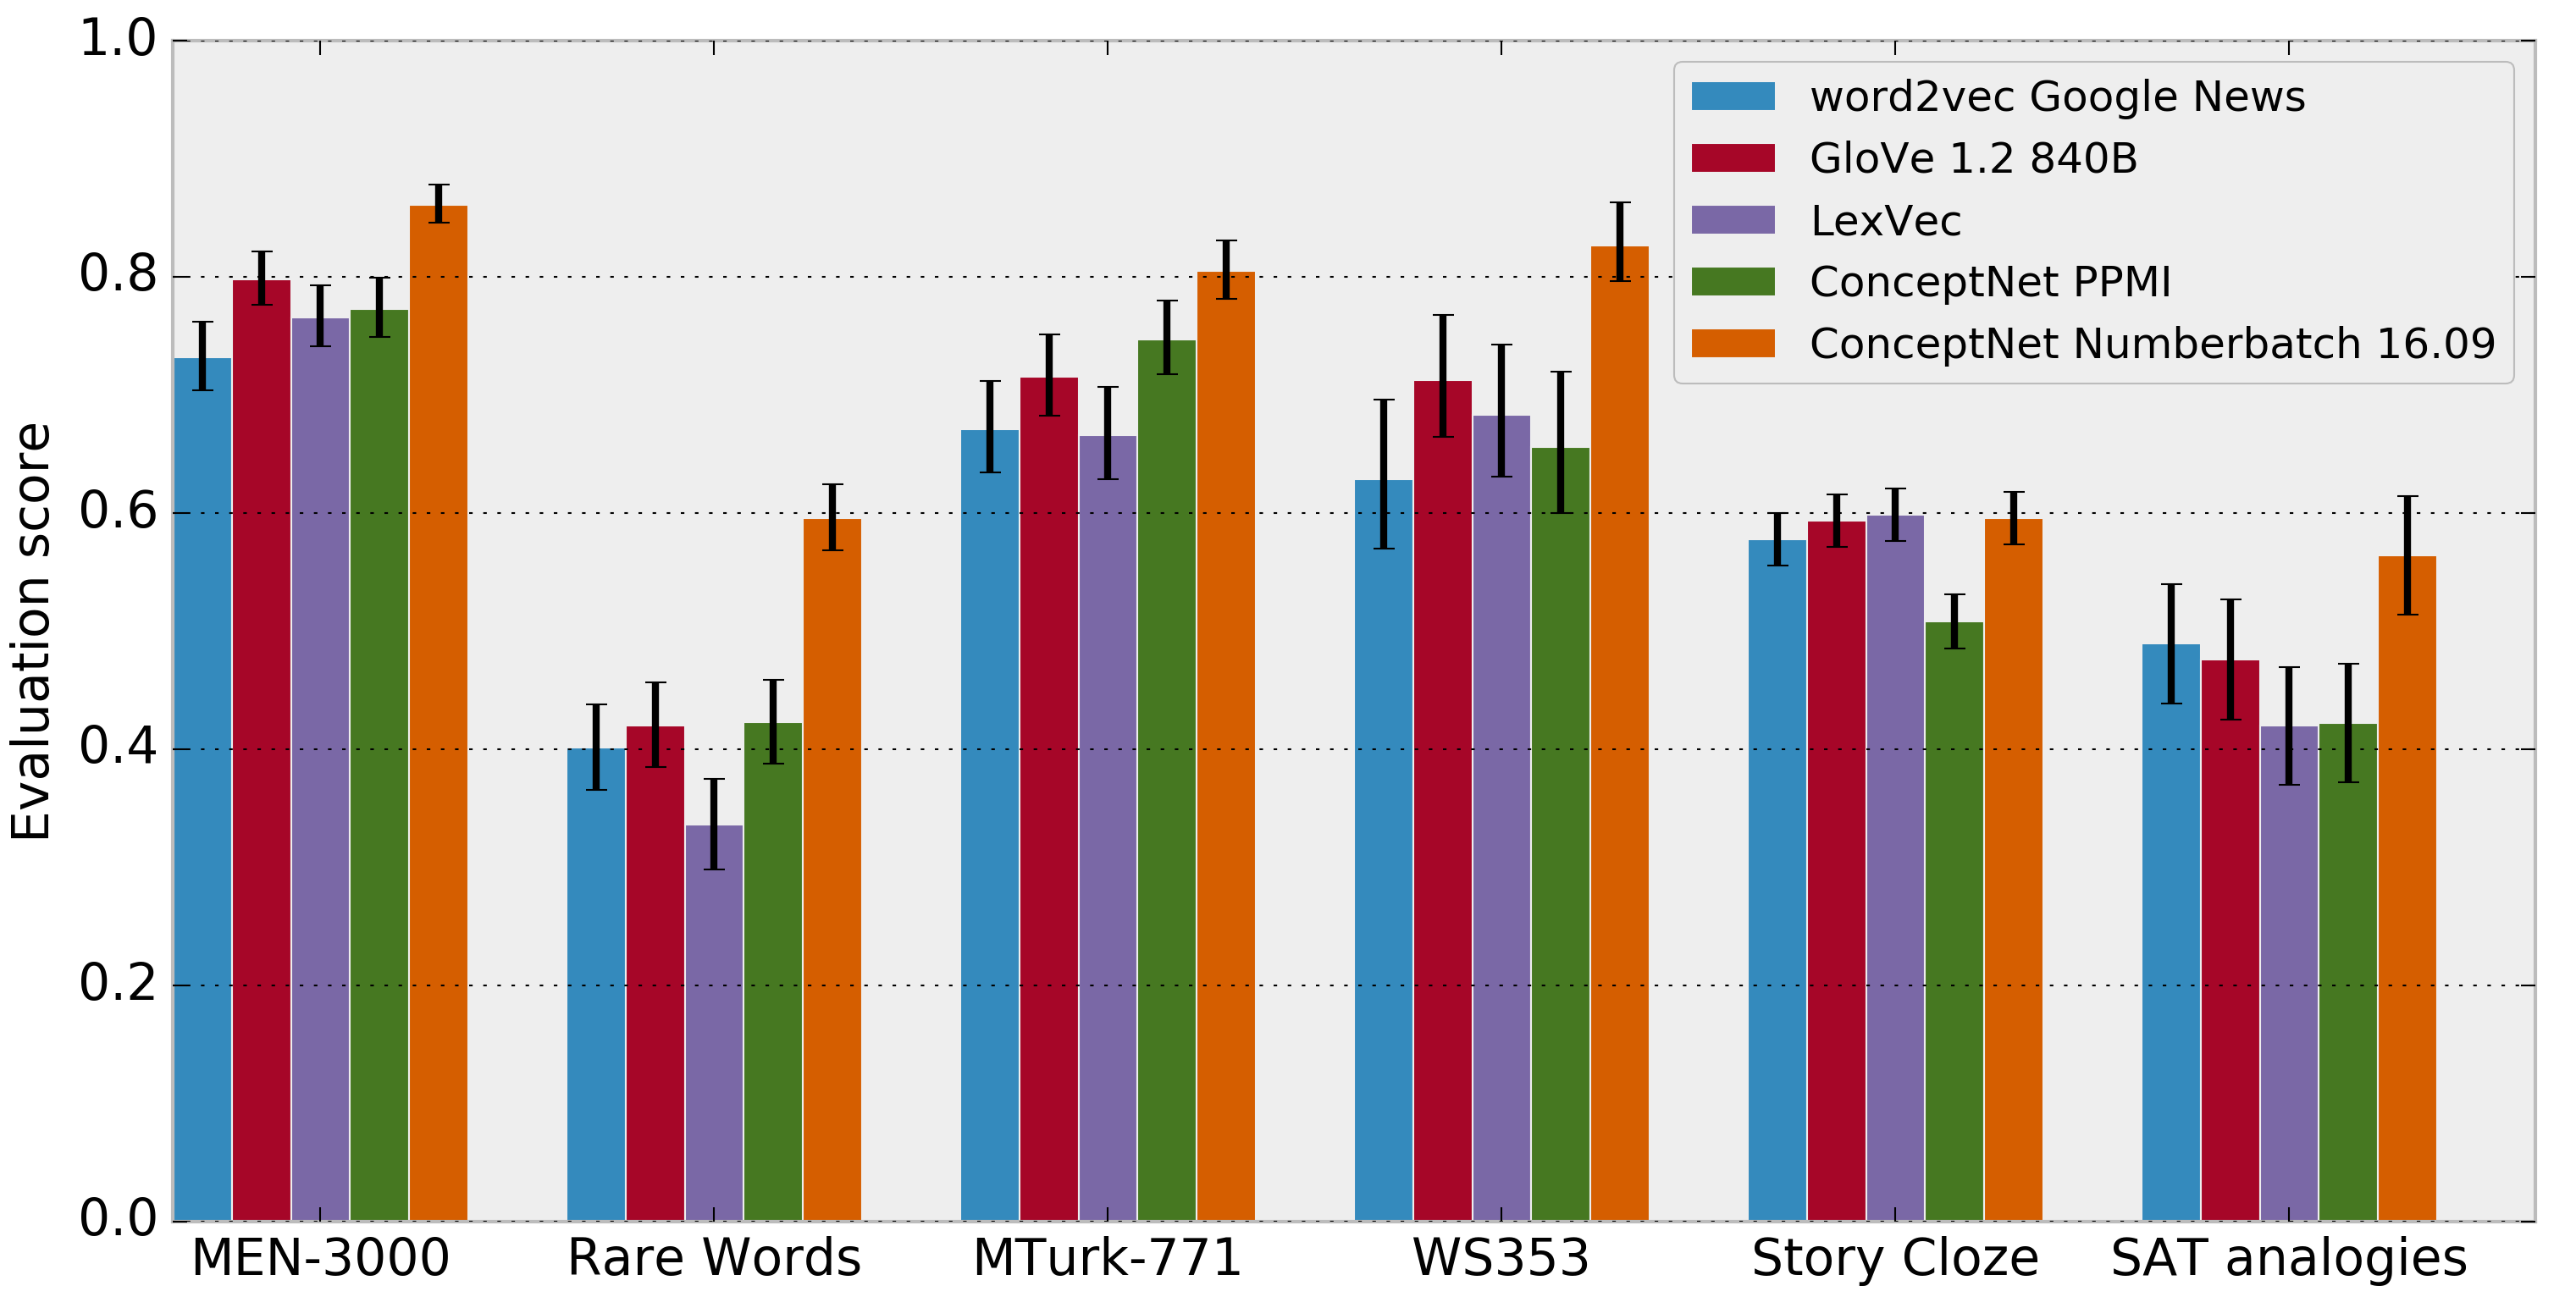
\includegraphics[width=3.3in]{eval-graph.png}
\caption{
    Performance across multiple evaluations of word embeddings built from
    ConceptNet, compared to other public word embeddings. Error bars
    show 95\% confidence intervals.
}
\label{eval-results}
\end{figure}

Figure~\ref{eval-results} compares the performance of the systems we compared
across all evaluations. For word-relatedness evaluations, the Y-axis represents
the Spearman correlation ($\rho$), using the Fisher transformation to compute a
95\% confidence interval that assumes the given word pairs are sampled from a
larger unobservable set \cite{bonett2000sample}. For the analogy and story evaluations,
the Y-axis is simply the proportion of questions answered correctly, with 95\%
confidence intervals calculated using the binomial exact test.

MEN-3000 and the Story Cloze Test have a standard development/test split, so
their data shows performance on the test data only.

On the four word-relatedness evaluations, ConceptNet Numberbatch 16.09 (the
complete system described in this paper) is state of the art, performing
significantly better than all other systems evaluated. Its high scores on both
the Rare Words dataset and the crowd-sourced MEN-3000 and MTurk-771 datasets
shows both the breadth and the depth of its understanding of words.

ConceptNet Numberbatch also performed the best at SAT analogies, getting 56.4\%
of the questions correct (57.0\% on the half that was held out for final
testing), with a 95\% confidence interval of 51.4\%--61.4\%.
This compares to LRA \cite{turney2005lra}, which scored 56.1\% and was
allowed to search AltaVista during the evaluation, as well as the previous best
self-contained system, SuperSim \cite{turney2013supersim}, which scored 54.8\%.
This also compares to the performance of the average human college applicant,
said by Turney and Littman to be 57.0\%.

The performance of our system on the Story Cloze Test was acceptable but
unremarkable.  ConceptNet Numberbatch chose the correct ending 59.5\% of the
time, which is in fact slightly better than any results reported by
\citeauthor{mostafazadeh2016cloze} \citeyear{mostafazadeh2016cloze}, including
neural nets trained on the task. However, we could also achieve a similar score
by using the same bag-of-vectors approach on other word embeddings. The best
score of 59.9\% was achieved by LexVec, with Numberbatch, GloVe, and word2vec
all within its margin of error.

The precise scores of our system on all these evaluations appear in
Table~\ref{eval-table}, including a development/test breakdown that shows no
noticeable overfitting.

% TODO: evaluation table

\subsection{Discussion of results}

\section{Availability of this code and data}

% TODO: make Zenodo citations for Numberbatch

The code for building and evaluating ConceptNet and its embeddings is part of
the ConceptNet 5 codebase, developed at \url{http://github.com/commonsense/conceptnet5}.
The version that produced this paper has been archived on the research repository
Zenodo at [FIXME]. The output embeddings, ConceptNet Numberbatch 2016.09, are similarly
archived at [FIXME].

\section{Acknowledgments}

\bibliographystyle{aaai}
\bibliography{conceptnet-paper}

\end{document}
